
\subsubsection{General description}
The netlist format has a simple line-based syntax.
Each line represents either a component or a connection between two components.
Lines that begin with a number sign (\texttt{\#}) are comments.
They are ignored by the parser, as are empty lines.
The whole netlist shares one common namespace.
Syntax elements with the same name thus refer to the same variable.
Any spaces and tabulators may be added for improving readability and will be ignored by the parser.

\subsubsection{Structure of a Description Line}
\label{sec_netlist_syntax}
\begin{figure}[Hbt]
	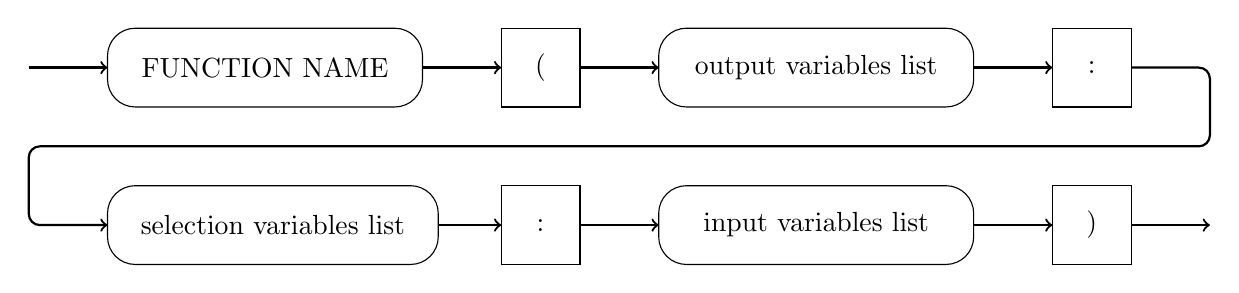
\begin{tikzpicture}
%
% syntax for a marconetlist line

%% opening
\draw[->, thick] (0,0) -- (1,0);
\draw[rounded corners=10] (1, -0.5) rectangle (5, 0.5);
	\node  at (3,0) {FUNCTION NAME};
\draw[->, thick] (5,0) -- (6,0);
\draw (6, -0.5) rectangle (7, 0.5);
	\node  at (6.5,0) {(};

\draw[->, thick] (7,0) -- (8,0);
\draw[rounded corners=10] (8, -0.5) rectangle (12, 0.5);
	\node  at (10,0) {output variables list};
\draw[->, thick] (12,0) -- (13,0);
\draw (13, -0.5) rectangle (14, 0.5);
	\node  at (13.5,0) {:};
%% linebreak
\draw[->, thick, rounded corners] (14,0) -- (15,0)--(15,-1)--(0,-1)--(0,-2)--(1,-2);
%% next line
\draw[rounded corners=10] (1, -2.5) rectangle (5.2, -1.5);
	\node  at (3.1,-2) {selection variables list};
\draw[->, thick] (5.2,-2) -- (6,-2);
\draw (6, -2.5) rectangle (7, -1.5);
	\node  at (6.5,-2) {:};
\draw[->, thick, rounded corners] (7,-2) -- (8,-2);
\draw[rounded corners=10] (8, -2.5) rectangle (12, -1.5);
	\node  at (10,-2) {input variables list};
\draw[->, thick] (12,-2) -- (13,-2);
\draw (13, -2.5) rectangle (14, -1.5);
	\node  at (13.5,-2) {)};
%% end
\draw[->, thick](14, -2)--(15,-2);
\end{tikzpicture}
	\caption{Syntax graph for a line in the intermediate netlist format}
		\label{img_line_syntax}
\end{figure}

As shown in figure \ref{img_line_syntax} a line describing a component or a connection between components is composed of a upper-case \texttt{FUNCTION NAME} and three variable lists in a certain order.

\begin{figure}[Hbt]
        \centering
        \begin{subfigure}[b]{0.4\textwidth}
               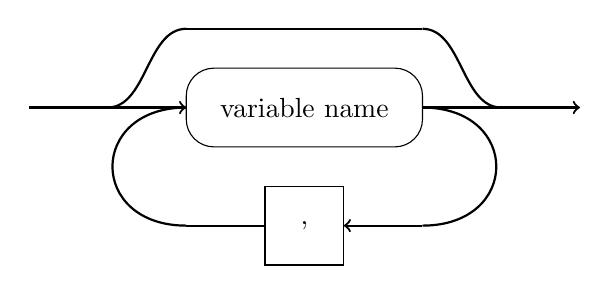
\begin{tikzpicture}
%\draw[style=help lines] (0,-1) grid (18,1);

\draw[->, thick] (0,0)--(2,0);
\draw[rounded corners=10] (2,-0.5) rectangle (5,0.5);
	\node at (3.5,0) {variable name};
\draw[->, thick] (5,0)--(7, 0);

% back loop
\draw[thick](5,0) .. controls (6.25,0) and (6.25,-1.5) .. (5,-1.5);
\draw[->, thick](5,-1.5)--(4,-1.5);
\draw(3,-2) rectangle (4,-1);
	\node at (3.5,-1.5){,};
\draw[thick](3,-1.5)--(2,-1.5);
\draw[thick](2,-1.5)  .. controls (0.75,-1.5) and (0.75,0) .. (2,0);

% bypass
\draw[thick] (1,0) .. controls (1.5,0) and (1.5,1) .. (2,1);
\draw[thick](2,1)--(5,1);
\draw[thick] (5,1) .. controls (5.5,1) and (5.5,0) .. (6,0);

\end{tikzpicture}
                \caption{Selection variables list}
                \label{img_var_syntax_mayempty}
        \end{subfigure}%
        \hfill %add desired spacing between images
        \begin{subfigure}[b]{0.4\textwidth}
                \input{diagrams/variable_list_nonempty_syntax.pgf}
                \caption{In- and Output variables list}
                \label{img_var_syntax_nonempty}
        \end{subfigure}
        \caption{Syntax graphs for the variables lists}
        \label{img_var_syntax}
\end{figure}

Each of these variable lists follows the structure given in figure \ref{img_var_syntax}.
Note, that the \texttt{selection variables lists} are allowed to be empty.
The naming of variables follows a strict structure.
Figure \ref{img_var_name_syntax} shows that it requires each component to be uniquely named. As a further restriction these \texttt{component names} may not contain whitespaces and must not begin with a number.

\begin{figure}[Hbt]
	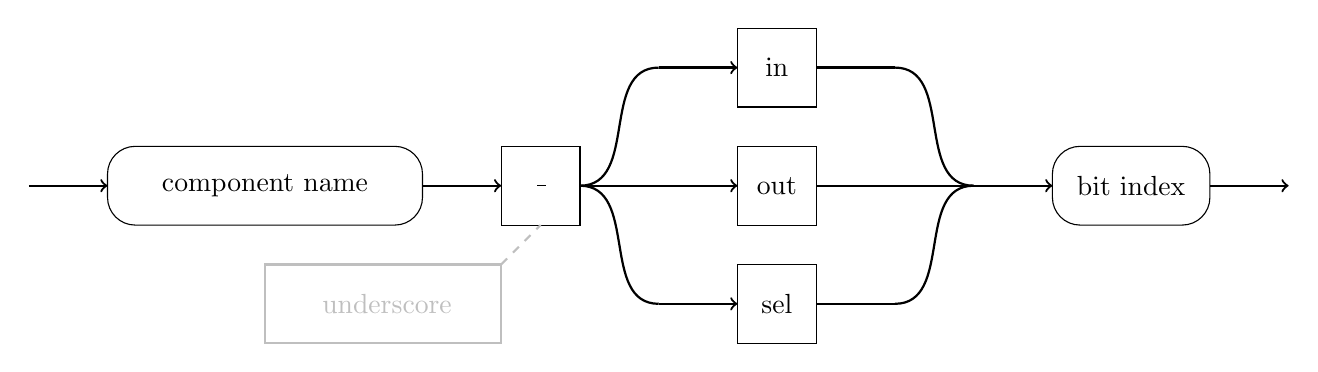
\begin{tikzpicture}
%\draw[style=help lines] (0,-1) grid (18,1);

\draw[->, thick] (0,0)--(1,0);
\draw[rounded corners=10] (1,-0.5) rectangle (5,0.5);
	\node at (3,0){component name};
\draw[->, thick] (5,0) -- (6,0);
\draw (6,-0.5) rectangle (7,0.5);
	\node at (6.5,0){\_};

% in
\draw[thick](7,0) .. controls (7.75,0) and (7.25,1.5) .. (8,1.5);
\draw[->, thick] (8,1.5)--(9,1.5);
\draw(9,1) rectangle (10,2);
	\node at (9.5,1.5) {in};
\draw[thick] (10,1.5)--(11,1.5);
\draw[thick](11,1.5) .. controls (11.75,1.5) and (11.25,0) .. (12,0);

% out
\draw[->, thick] (7,0)--(9,0);
\draw(9,-0.5) rectangle (10,0.5);
	\node at (9.5,0) {out};
\draw[->, thick] (10,0)--(13,0);

% sel
\draw[thick](7,0) .. controls (7.75,0) and (7.25,-1.5) .. (8,-1.5);
\draw[->, thick] (8,-1.5)--(9,-1.5);
\draw(9,-2) rectangle (10,-1);
	\node at (9.5,-1.5) {sel};
\draw[thick] (10,-1.5)--(11,-1.5);
\draw[thick](11,-1.5) .. controls (11.75,-1.5) and (11.25,0) .. (12,0);

\draw[rounded corners=10] (13,-0.5) rectangle (15,0.5);
	\node at (14,0){bit index};

\draw[->, thick] (15,0)--(16,0);

% annotation
\draw[thick, lightgray, dashed](6,-1)--(6.5,-0.5);
\draw[thick, lightgray] (3,-2) rectangle (6,-1);
	\node[lightgray] at (4.55,-1.5){underscore};
\end{tikzpicture}
	\caption{Syntax graph for the variable name}
		\label{img_var_name_syntax}
\end{figure}

The \texttt{bit indices} of the variables are natural numbers. 
Given, there where $n$ variables in a variables list, they would have the \texttt{bit indices} from $n-1$ to $0$.
Variables are ordered from highest to lowest \texttt{bit index} in each of the variables lists.

\subsubsection{Semantics of a Description Line}
Each of the lines following the specification given above describes either a component or the connection between components.
Each variable in the variables lists is associated with one bit of a components ports.
These bits are ordered first by meaning and thereafter by significance.
The meaning decides in which of the variables lists a variable is put. Their meaning also influences the variable names infix as provided by figure \ref{img_var_name_syntax}:
\begin{description}
	\item[Input] direction variables provide data for a component to operate with. This is determined by the infix \texttt{in}.
	\item[Output] direction variables represent the result of a components operation. They are infixed with \texttt{out}.
		\item[Selection] variables are a special case of input variables. They are meaningful for components that can choose between different ways of operation, depending on a given configuration. These configurations can be given by manipulation the selection variables. They are marked by the infix \texttt{sel}.
\end{description}
Significance of a bit is expressed by the associated variables index. The order is from highest significance to lowest. 
Combined with the restriction given in section \ref{sec_netlist_syntax} it follows that the \gls{msb} has index $n-1$ and the \gls{lsb} ist indexed with $0$.

The \texttt{FUNCTION NAME} corresponds with the function of the component and may be of the following:
\begin{itemize}
	\item A boolean function, which is one of 
		\texttt{NOT},
		\texttt{AND},
		\texttt{NAND},
		\texttt{OR} or
		\texttt{NOR}
		%% support XOR / XNOR?
		%% support TRUE / FALSE ?
		%% support Buffer ?
	\item A multiplexer, denoted as \texttt{MUX}
	\item A lookup table, denoted as \texttt{LUT}
\end{itemize}

Connections between components are represented by the function \texttt{CONNECT}. They are the only cases in which the \texttt{component names} of the variables may differ, even if in the same variables list.

Intermediate nodes that just result from wire routing or forking wires are named as shown in %% TODO fig
A nodes index is an incremental natural number beginning at $0$.
The order in which nodes are indexed is arbitrary.

\subsubsection{Example of a simple Netlist}